% !TeX root = ../Harte_Kugeln.tex
\todo{Tabelle einfügen mit Werten von Experiment. Anzahl Teilchen; Anfangsbedingungen, Aufwärmen; wieviele Stöße; welche Dichten untersucht; reduzierte Größen ($T^*=1$)}
Um eine statistische Auswertung der zu untersuchenden Eigenschaften zu ermöglichen, wurden die zu erhebenden Daten in konstanten Zeitabständen berechnet und gespeichert. Da die Simulation aber in nicht-konstanten Zeitschritten voranschreitet, wurde vor jedem neuen Stoß ermittelt, ob zwischen dem neuen und dem letzten ein Daten-Sampling stattfinden sollte. Falls dem so wäre, wurde die Zeit des Systems bis zum Auswertungszeitpunkt ``vorgespult'' --- sprich: alle Kugeln ballistisch für die Zeit $\Delta t$ bewegt ---, die Ergebnisse in ein File geschrieben und erst anschließend der Stoß durchgeführt.   
\subsection{Paarverteilungsfunktion}\label{sec:paarverteilung}
Eine Flüssigkeit oder ein Gas mit rein additiven Paarwechselwirkungen kann durch die sogenannte Paarverteilungsfunktion --- manchmal auch Paarkorrelationsfunktion oder radiale Verteilungsfunktion --- $g(r)$ vollständig charakterisiert werden. Diese Funktion gibt Aufschluss über die kurzreichweitige Struktur des Fluids --- also seine Nahordnung. Sie beschreibt die Häufigkeit, mit der sich zwei Teilchen in einem gewissen Abstand $r$ voneinander entfernt befinden, bezogen auf die jeweilige Häufigkeit in einem idealen Gas. Die Paarverteilungsfunktion ist demnach gegeben durch
 
 \begin{equation}
g(r) = \frac{1}{4\pi r^2 \rho N}\langle \sum_{j\neq i} \delta(r-r_{ij}) \rangle
\end{equation}
Da Fluide keine Fernordnung besitzen, muss die Paarverteilungsfunktion im Limes $r \rightarrow \infty$ gegen 1 konvergieren. Des weiteren sei angemerkt, dass die Paarverteilungsfunktion der Randverteilung der $N$-Teilchen-Wahrscheinlichkeitsdichte entspricht und man demnach im Limes $\rho \rightarrow 0$ direkt das Paarpotential $U(r)$ aus der Paarverteilungsfunktion ablesen kann.  
\begin{equation}
\lim_{\rho \rightarrow 0} g(r) = e^{-\beta U(r)}
\end{equation}
Für Festkörper lässt sich natürlich auch eine Paarverteilungsfunktion definieren, allerdings ist diese nicht mehr isotrop sondern richtungsabhängig. 
\begin{equation}
g(\vec{r}) = \frac{1}{\rho N} \langle \sum_{j\neq i} \delta^{(3)}(\vec{r}-\vec{r_{ij}}) \rangle
\end{equation} 
Häufig wird aber auch die winkelgemittelte Version verwendet, welche dann mit der Definition der Paarverteilungsfunktion für Fluide übereinstimmt. 

Abbildungen \ref{fig:paarverteilung1}, \ref{fig:paarverteilung2} und \ref{fig:paarverteilung3} zeigen die Paarverteilungsfunktionen des Systems von harten Kugeln für verschiedene Dichten $\rho$ von 0.2 bis 1.3. Die Entstehung von Nahordnung beim Übergang vom gasförmigen zum flüssigen Zustand mit zunehmender Dichte lässt sich gut anhand von Abbildung \ref{fig:paarverteilung1} erkennen. Im ungeordneten (gasförmigen) Zustand nimmt die Paarverteilungsfunktion mit der Entfernung monoton ab, während sich beim Phasenübergang zur Flüssigkeit ein zweites Maximum ausbildet. 

\begin{figure}[H]
 \centering
 \resizebox{0.9\textwidth}{!}{% GNUPLOT: LaTeX picture with Postscript
\begingroup
  \makeatletter
  \providecommand\color[2][]{%
    \GenericError{(gnuplot) \space\space\space\@spaces}{%
      Package color not loaded in conjunction with
      terminal option `colourtext'%
    }{See the gnuplot documentation for explanation.%
    }{Either use 'blacktext' in gnuplot or load the package
      color.sty in LaTeX.}%
    \renewcommand\color[2][]{}%
  }%
  \providecommand\includegraphics[2][]{%
    \GenericError{(gnuplot) \space\space\space\@spaces}{%
      Package graphicx or graphics not loaded%
    }{See the gnuplot documentation for explanation.%
    }{The gnuplot epslatex terminal needs graphicx.sty or graphics.sty.}%
    \renewcommand\includegraphics[2][]{}%
  }%
  \providecommand\rotatebox[2]{#2}%
  \@ifundefined{ifGPcolor}{%
    \newif\ifGPcolor
    \GPcolortrue
  }{}%
  \@ifundefined{ifGPblacktext}{%
    \newif\ifGPblacktext
    \GPblacktextfalse
  }{}%
  % define a \g@addto@macro without @ in the name:
  \let\gplgaddtomacro\g@addto@macro
  % define empty templates for all commands taking text:
  \gdef\gplbacktext{}%
  \gdef\gplfronttext{}%
  \makeatother
  \ifGPblacktext
    % no textcolor at all
    \def\colorrgb#1{}%
    \def\colorgray#1{}%
  \else
    % gray or color?
    \ifGPcolor
      \def\colorrgb#1{\color[rgb]{#1}}%
      \def\colorgray#1{\color[gray]{#1}}%
      \expandafter\def\csname LTw\endcsname{\color{white}}%
      \expandafter\def\csname LTb\endcsname{\color{black}}%
      \expandafter\def\csname LTa\endcsname{\color{black}}%
      \expandafter\def\csname LT0\endcsname{\color[rgb]{1,0,0}}%
      \expandafter\def\csname LT1\endcsname{\color[rgb]{0,1,0}}%
      \expandafter\def\csname LT2\endcsname{\color[rgb]{0,0,1}}%
      \expandafter\def\csname LT3\endcsname{\color[rgb]{1,0,1}}%
      \expandafter\def\csname LT4\endcsname{\color[rgb]{0,1,1}}%
      \expandafter\def\csname LT5\endcsname{\color[rgb]{1,1,0}}%
      \expandafter\def\csname LT6\endcsname{\color[rgb]{0,0,0}}%
      \expandafter\def\csname LT7\endcsname{\color[rgb]{1,0.3,0}}%
      \expandafter\def\csname LT8\endcsname{\color[rgb]{0.5,0.5,0.5}}%
    \else
      % gray
      \def\colorrgb#1{\color{black}}%
      \def\colorgray#1{\color[gray]{#1}}%
      \expandafter\def\csname LTw\endcsname{\color{white}}%
      \expandafter\def\csname LTb\endcsname{\color{black}}%
      \expandafter\def\csname LTa\endcsname{\color{black}}%
      \expandafter\def\csname LT0\endcsname{\color{black}}%
      \expandafter\def\csname LT1\endcsname{\color{black}}%
      \expandafter\def\csname LT2\endcsname{\color{black}}%
      \expandafter\def\csname LT3\endcsname{\color{black}}%
      \expandafter\def\csname LT4\endcsname{\color{black}}%
      \expandafter\def\csname LT5\endcsname{\color{black}}%
      \expandafter\def\csname LT6\endcsname{\color{black}}%
      \expandafter\def\csname LT7\endcsname{\color{black}}%
      \expandafter\def\csname LT8\endcsname{\color{black}}%
    \fi
  \fi
  \setlength{\unitlength}{0.0500bp}%
  \begin{picture}(8502.00,6802.00)%
    \gplgaddtomacro\gplbacktext{%
      \csname LTb\endcsname%
      \put(946,704){\makebox(0,0)[r]{\strut{} 0.8}}%
      \put(946,1537){\makebox(0,0)[r]{\strut{} 1}}%
      \put(946,2371){\makebox(0,0)[r]{\strut{} 1.2}}%
      \put(946,3204){\makebox(0,0)[r]{\strut{} 1.4}}%
      \put(946,4037){\makebox(0,0)[r]{\strut{} 1.6}}%
      \put(946,4870){\makebox(0,0)[r]{\strut{} 1.8}}%
      \put(946,5704){\makebox(0,0)[r]{\strut{} 2}}%
      \put(946,6537){\makebox(0,0)[r]{\strut{} 2.2}}%
      \put(1078,484){\makebox(0,0){\strut{} 1}}%
      \put(2483,484){\makebox(0,0){\strut{} 1.5}}%
      \put(3889,484){\makebox(0,0){\strut{} 2}}%
      \put(5294,484){\makebox(0,0){\strut{} 2.5}}%
      \put(6700,484){\makebox(0,0){\strut{} 3}}%
      \put(8105,484){\makebox(0,0){\strut{} 3.5}}%
      \put(176,3620){\rotatebox{-270}{\makebox(0,0){\strut{}$g(r)$}}}%
      \put(4591,154){\makebox(0,0){\strut{}$r [\text{m}]$}}%
    }%
    \gplgaddtomacro\gplfronttext{%
      \csname LTb\endcsname%
      \put(7118,6364){\makebox(0,0)[r]{\strut{}$\rho$ = 0.2}}%
      \csname LTb\endcsname%
      \put(7118,6144){\makebox(0,0)[r]{\strut{}$\rho$ = 0.3}}%
      \csname LTb\endcsname%
      \put(7118,5924){\makebox(0,0)[r]{\strut{}$\rho$ = 0.4}}%
      \csname LTb\endcsname%
      \put(7118,5704){\makebox(0,0)[r]{\strut{}$\rho$ = 0.5}}%
    }%
    \gplbacktext
    \put(0,0){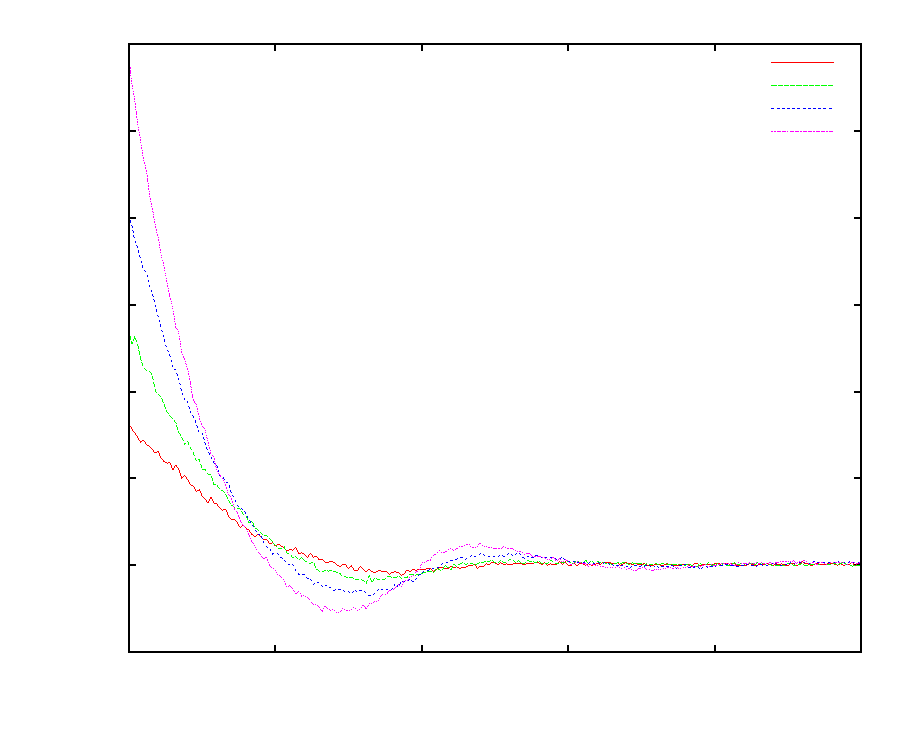
\includegraphics{PairDistribution1}}%
    \gplfronttext
  \end{picture}%
\endgroup
}
 \caption{Paarverteilungsfunktion für verschiedene Dichten $\rho$ im Bereich von 0.2 bis 0.5 (fluid)}
 \label{fig:paarverteilung1}
\end{figure} 

Harte Kugeln durchlaufen einen Phasenübergang vom fluiden zum festen Zustand zwischen Packungsdichten von $n_f \approx 0.494$ und $n_s \approx 0.545$\todo{[citation needed]}, was den reduzierten Dichten $\rho_f \approx 0.943$ und $\rho_s \approx 1.041$ entspricht. Anhand von Abbildungen \ref{fig:paarverteilung2} und \ref{fig:paarverteilung3} kann man diesen Phasenübergang deutlich erkennen --- die Maxima werden immer prominenter, was auf eine geordnete Kristallstruktur schließen lässt. 
 
\begin{figure}[H]
 \centering
 \resizebox{0.9\textwidth}{!}{% GNUPLOT: LaTeX picture with Postscript
\begingroup
  \makeatletter
  \providecommand\color[2][]{%
    \GenericError{(gnuplot) \space\space\space\@spaces}{%
      Package color not loaded in conjunction with
      terminal option `colourtext'%
    }{See the gnuplot documentation for explanation.%
    }{Either use 'blacktext' in gnuplot or load the package
      color.sty in LaTeX.}%
    \renewcommand\color[2][]{}%
  }%
  \providecommand\includegraphics[2][]{%
    \GenericError{(gnuplot) \space\space\space\@spaces}{%
      Package graphicx or graphics not loaded%
    }{See the gnuplot documentation for explanation.%
    }{The gnuplot epslatex terminal needs graphicx.sty or graphics.sty.}%
    \renewcommand\includegraphics[2][]{}%
  }%
  \providecommand\rotatebox[2]{#2}%
  \@ifundefined{ifGPcolor}{%
    \newif\ifGPcolor
    \GPcolortrue
  }{}%
  \@ifundefined{ifGPblacktext}{%
    \newif\ifGPblacktext
    \GPblacktextfalse
  }{}%
  % define a \g@addto@macro without @ in the name:
  \let\gplgaddtomacro\g@addto@macro
  % define empty templates for all commands taking text:
  \gdef\gplbacktext{}%
  \gdef\gplfronttext{}%
  \makeatother
  \ifGPblacktext
    % no textcolor at all
    \def\colorrgb#1{}%
    \def\colorgray#1{}%
  \else
    % gray or color?
    \ifGPcolor
      \def\colorrgb#1{\color[rgb]{#1}}%
      \def\colorgray#1{\color[gray]{#1}}%
      \expandafter\def\csname LTw\endcsname{\color{white}}%
      \expandafter\def\csname LTb\endcsname{\color{black}}%
      \expandafter\def\csname LTa\endcsname{\color{black}}%
      \expandafter\def\csname LT0\endcsname{\color[rgb]{1,0,0}}%
      \expandafter\def\csname LT1\endcsname{\color[rgb]{0,1,0}}%
      \expandafter\def\csname LT2\endcsname{\color[rgb]{0,0,1}}%
      \expandafter\def\csname LT3\endcsname{\color[rgb]{1,0,1}}%
      \expandafter\def\csname LT4\endcsname{\color[rgb]{0,1,1}}%
      \expandafter\def\csname LT5\endcsname{\color[rgb]{1,1,0}}%
      \expandafter\def\csname LT6\endcsname{\color[rgb]{0,0,0}}%
      \expandafter\def\csname LT7\endcsname{\color[rgb]{1,0.3,0}}%
      \expandafter\def\csname LT8\endcsname{\color[rgb]{0.5,0.5,0.5}}%
    \else
      % gray
      \def\colorrgb#1{\color{black}}%
      \def\colorgray#1{\color[gray]{#1}}%
      \expandafter\def\csname LTw\endcsname{\color{white}}%
      \expandafter\def\csname LTb\endcsname{\color{black}}%
      \expandafter\def\csname LTa\endcsname{\color{black}}%
      \expandafter\def\csname LT0\endcsname{\color{black}}%
      \expandafter\def\csname LT1\endcsname{\color{black}}%
      \expandafter\def\csname LT2\endcsname{\color{black}}%
      \expandafter\def\csname LT3\endcsname{\color{black}}%
      \expandafter\def\csname LT4\endcsname{\color{black}}%
      \expandafter\def\csname LT5\endcsname{\color{black}}%
      \expandafter\def\csname LT6\endcsname{\color{black}}%
      \expandafter\def\csname LT7\endcsname{\color{black}}%
      \expandafter\def\csname LT8\endcsname{\color{black}}%
    \fi
  \fi
  \setlength{\unitlength}{0.0500bp}%
  \begin{picture}(8502.00,6802.00)%
    \gplgaddtomacro\gplbacktext{%
      \csname LTb\endcsname%
      \put(946,704){\makebox(0,0)[r]{\strut{} 0.5}}%
      \put(946,1287){\makebox(0,0)[r]{\strut{} 1}}%
      \put(946,1871){\makebox(0,0)[r]{\strut{} 1.5}}%
      \put(946,2454){\makebox(0,0)[r]{\strut{} 2}}%
      \put(946,3037){\makebox(0,0)[r]{\strut{} 2.5}}%
      \put(946,3621){\makebox(0,0)[r]{\strut{} 3}}%
      \put(946,4204){\makebox(0,0)[r]{\strut{} 3.5}}%
      \put(946,4787){\makebox(0,0)[r]{\strut{} 4}}%
      \put(946,5370){\makebox(0,0)[r]{\strut{} 4.5}}%
      \put(946,5954){\makebox(0,0)[r]{\strut{} 5}}%
      \put(946,6537){\makebox(0,0)[r]{\strut{} 5.5}}%
      \put(1078,484){\makebox(0,0){\strut{} 1}}%
      \put(2483,484){\makebox(0,0){\strut{} 1.5}}%
      \put(3889,484){\makebox(0,0){\strut{} 2}}%
      \put(5294,484){\makebox(0,0){\strut{} 2.5}}%
      \put(6700,484){\makebox(0,0){\strut{} 3}}%
      \put(8105,484){\makebox(0,0){\strut{} 3.5}}%
      \put(176,3620){\rotatebox{-270}{\makebox(0,0){\strut{}$g(r)$}}}%
      \put(4591,154){\makebox(0,0){\strut{}$r [\text{m}]$}}%
    }%
    \gplgaddtomacro\gplfronttext{%
      \csname LTb\endcsname%
      \put(7118,6364){\makebox(0,0)[r]{\strut{}$\rho$ = 0.6}}%
      \csname LTb\endcsname%
      \put(7118,6144){\makebox(0,0)[r]{\strut{}$\rho$ = 0.7}}%
      \csname LTb\endcsname%
      \put(7118,5924){\makebox(0,0)[r]{\strut{}$\rho$ = 0.8}}%
      \csname LTb\endcsname%
      \put(7118,5704){\makebox(0,0)[r]{\strut{}$\rho$ = 0.9}}%
    }%
    \gplbacktext
    \put(0,0){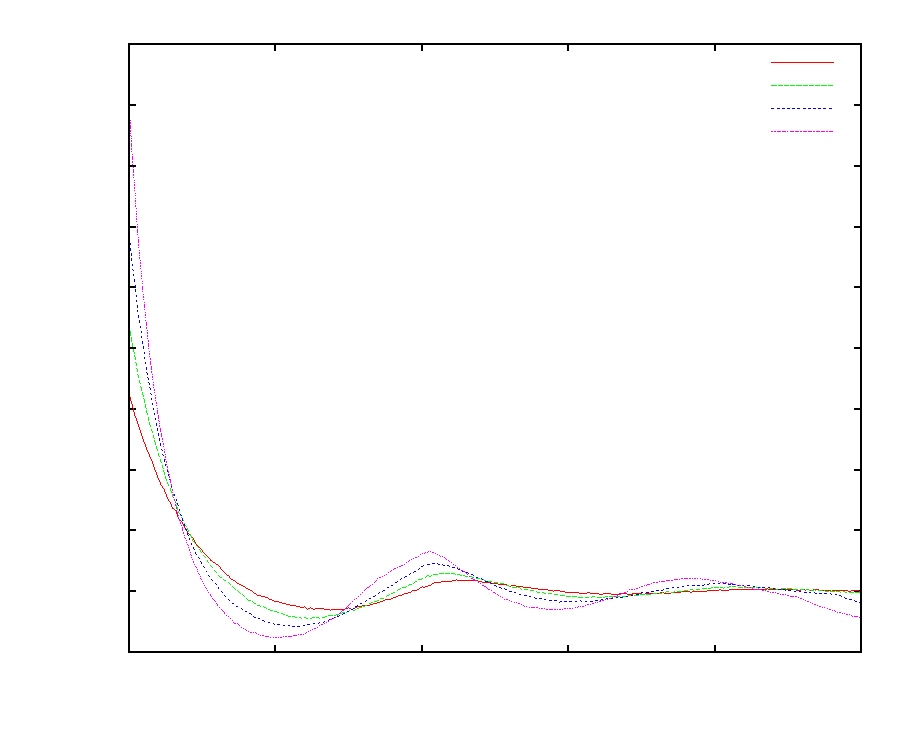
\includegraphics{PairDistribution5}}%
    \gplfronttext
  \end{picture}%
\endgroup
}
  \caption{Paarverteilungsfunktion für verschiedene Dichten $\rho$ im Bereich von 0.6 bis 0.9 (fluid) }
 \label{fig:paarverteilung2}
\end{figure} 
 
Theoretisch sollte ein System von harten Kugeln ein fcc-Kristallgitter ausbilden indem die einzelnen Kugeln einen relativen Abstand von $r_1 : r_2 : r_3 = 1 : \sqrt{2} : \sqrt{3}$ zu ihren nächsten Nachbarn aufweisen. Bei einer Dichte von 1.3 finden sich die Maxima der Paarverteilungsfunktion auch ziemlich genau in diesen Abständen. 
 

\begin{figure}[H]
 \centering
  \resizebox{0.9\textwidth}{!}{% GNUPLOT: LaTeX picture with Postscript
\begingroup
  \makeatletter
  \providecommand\color[2][]{%
    \GenericError{(gnuplot) \space\space\space\@spaces}{%
      Package color not loaded in conjunction with
      terminal option `colourtext'%
    }{See the gnuplot documentation for explanation.%
    }{Either use 'blacktext' in gnuplot or load the package
      color.sty in LaTeX.}%
    \renewcommand\color[2][]{}%
  }%
  \providecommand\includegraphics[2][]{%
    \GenericError{(gnuplot) \space\space\space\@spaces}{%
      Package graphicx or graphics not loaded%
    }{See the gnuplot documentation for explanation.%
    }{The gnuplot epslatex terminal needs graphicx.sty or graphics.sty.}%
    \renewcommand\includegraphics[2][]{}%
  }%
  \providecommand\rotatebox[2]{#2}%
  \@ifundefined{ifGPcolor}{%
    \newif\ifGPcolor
    \GPcolortrue
  }{}%
  \@ifundefined{ifGPblacktext}{%
    \newif\ifGPblacktext
    \GPblacktextfalse
  }{}%
  % define a \g@addto@macro without @ in the name:
  \let\gplgaddtomacro\g@addto@macro
  % define empty templates for all commands taking text:
  \gdef\gplbacktext{}%
  \gdef\gplfronttext{}%
  \makeatother
  \ifGPblacktext
    % no textcolor at all
    \def\colorrgb#1{}%
    \def\colorgray#1{}%
  \else
    % gray or color?
    \ifGPcolor
      \def\colorrgb#1{\color[rgb]{#1}}%
      \def\colorgray#1{\color[gray]{#1}}%
      \expandafter\def\csname LTw\endcsname{\color{white}}%
      \expandafter\def\csname LTb\endcsname{\color{black}}%
      \expandafter\def\csname LTa\endcsname{\color{black}}%
      \expandafter\def\csname LT0\endcsname{\color[rgb]{1,0,0}}%
      \expandafter\def\csname LT1\endcsname{\color[rgb]{0,1,0}}%
      \expandafter\def\csname LT2\endcsname{\color[rgb]{0,0,1}}%
      \expandafter\def\csname LT3\endcsname{\color[rgb]{1,0,1}}%
      \expandafter\def\csname LT4\endcsname{\color[rgb]{0,1,1}}%
      \expandafter\def\csname LT5\endcsname{\color[rgb]{1,1,0}}%
      \expandafter\def\csname LT6\endcsname{\color[rgb]{0,0,0}}%
      \expandafter\def\csname LT7\endcsname{\color[rgb]{1,0.3,0}}%
      \expandafter\def\csname LT8\endcsname{\color[rgb]{0.5,0.5,0.5}}%
    \else
      % gray
      \def\colorrgb#1{\color{black}}%
      \def\colorgray#1{\color[gray]{#1}}%
      \expandafter\def\csname LTw\endcsname{\color{white}}%
      \expandafter\def\csname LTb\endcsname{\color{black}}%
      \expandafter\def\csname LTa\endcsname{\color{black}}%
      \expandafter\def\csname LT0\endcsname{\color{black}}%
      \expandafter\def\csname LT1\endcsname{\color{black}}%
      \expandafter\def\csname LT2\endcsname{\color{black}}%
      \expandafter\def\csname LT3\endcsname{\color{black}}%
      \expandafter\def\csname LT4\endcsname{\color{black}}%
      \expandafter\def\csname LT5\endcsname{\color{black}}%
      \expandafter\def\csname LT6\endcsname{\color{black}}%
      \expandafter\def\csname LT7\endcsname{\color{black}}%
      \expandafter\def\csname LT8\endcsname{\color{black}}%
    \fi
  \fi
  \setlength{\unitlength}{0.0500bp}%
  \begin{picture}(8502.00,6802.00)%
    \gplgaddtomacro\gplbacktext{%
      \csname LTb\endcsname%
      \put(814,704){\makebox(0,0)[r]{\strut{} 0}}%
      \put(814,1433){\makebox(0,0)[r]{\strut{} 2}}%
      \put(814,2162){\makebox(0,0)[r]{\strut{} 4}}%
      \put(814,2891){\makebox(0,0)[r]{\strut{} 6}}%
      \put(814,3621){\makebox(0,0)[r]{\strut{} 8}}%
      \put(814,4350){\makebox(0,0)[r]{\strut{} 10}}%
      \put(814,5079){\makebox(0,0)[r]{\strut{} 12}}%
      \put(814,5808){\makebox(0,0)[r]{\strut{} 14}}%
      \put(814,6537){\makebox(0,0)[r]{\strut{} 16}}%
      \put(946,484){\makebox(0,0){\strut{} 1}}%
      \put(2378,484){\makebox(0,0){\strut{} 1.5}}%
      \put(3810,484){\makebox(0,0){\strut{} 2}}%
      \put(5241,484){\makebox(0,0){\strut{} 2.5}}%
      \put(6673,484){\makebox(0,0){\strut{} 3}}%
      \put(8105,484){\makebox(0,0){\strut{} 3.5}}%
      \put(176,3620){\rotatebox{-270}{\makebox(0,0){\strut{}$g(r)$}}}%
      \put(4525,154){\makebox(0,0){\strut{}$r [\text{m}]$}}%
    }%
    \gplgaddtomacro\gplfronttext{%
      \csname LTb\endcsname%
      \put(7118,6364){\makebox(0,0)[r]{\strut{}$\rho$ = 1.0}}%
      \csname LTb\endcsname%
      \put(7118,6144){\makebox(0,0)[r]{\strut{}$\rho$ = 1.1}}%
      \csname LTb\endcsname%
      \put(7118,5924){\makebox(0,0)[r]{\strut{}$\rho$ = 1.2}}%
      \csname LTb\endcsname%
      \put(7118,5704){\makebox(0,0)[r]{\strut{}$\rho$ = 1.3}}%
    }%
    \gplbacktext
    \put(0,0){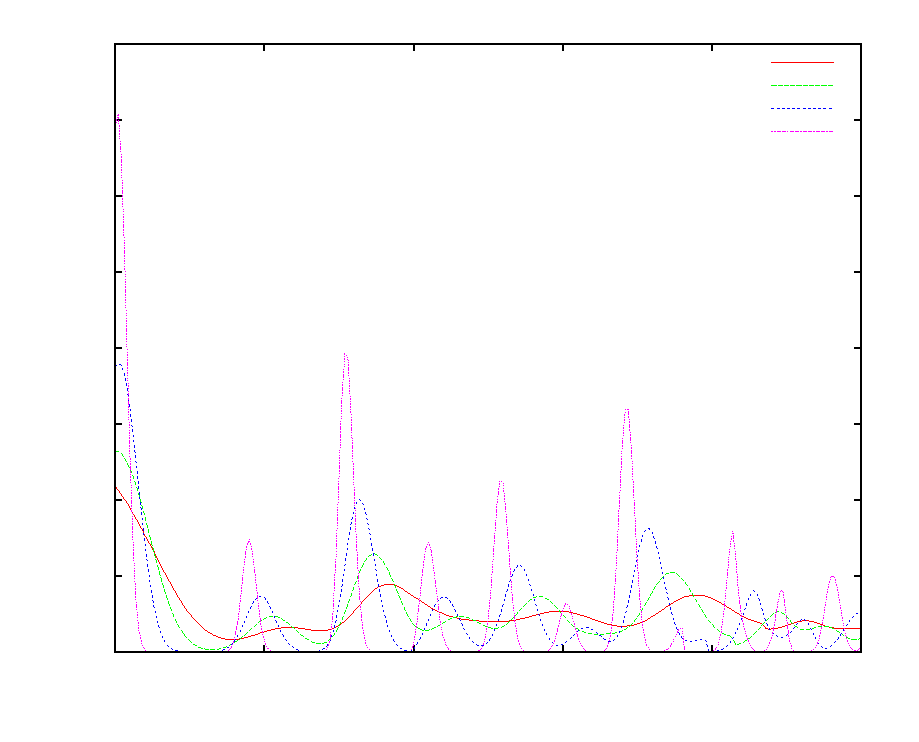
\includegraphics{PairDistribution9}}%
    \gplfronttext
  \end{picture}%
\endgroup
}
 \caption{Paarverteilungsfunktion für verschiedene Dichten $\rho$ im Bereich von 1.0 bis 1.3 (fest) }
 \label{fig:paarverteilung3}
\end{figure} 
  \todo{Simulation bei $\rho \approx 1.0$ fragwürdig weil Zweiphasenbereich}

\subsection{Thermische Zustandsgleichung}
Die Thermische Zustandsgleichung stellt einen Zusammenhang zwischen den Variablen Druck $p$, Temperatur $T$ und Dichte $\rho$ her. Sie kann mittels mehrerer Methoden berechnet werden. Die wohl am häufigsten verwendete bedient sich des Virials $W$  

\todo{ein minus zu viel. und irgendwas mit ``eigentlich der mittelwert'' beim $W$ term}
\begin{equation}
\frac{p}{\rho k T} = 1 - \frac{1}{3NkT}\underbrace{\sum_{i=1}^N \vec{r}_i \cdot \vec{F}_i}_{= - W}
\end{equation}
Alternativ kann diese Zustandsgleichung auch geschrieben werden als 
\begin{equation}
\frac{p}{\rho k T} = 1 - \frac{2\pi\rho}{3kT} \int_0^{\infty} \text{dr} r^2 g(r) r U'(r)  
\label{eos2}
\end{equation}
Da harte Kugeln allerdings ein nicht-differenzierbares Potential besitzen und demnach keine Kraft auf sie wirkt, solange sie nicht aneinander stoßen, muss die Berechnung der Zustandsgleichung für harte Kugeln etwas abgeändert werden.
Zu diesem Zweck sieht man ein System harter Kugeln als den Grenzfall eines Systems "`weicher Kugeln"' mit dem Potential 
\begin{equation}
U_{soft}(r) = \epsilon \left(\frac{\sigma}{r}\right)^n 
\end{equation}
an, welches sich im Limes $n \rightarrow \infty$ dem Potential harter Kugeln annähert. Der Boltzmannfaktor für dieses Potential nähert sich bei $n \rightarrow \infty$ einer Stufenfunktion an
\begin{equation}
e^{-\beta U_{soft}(r)} \rightarrow H(r-\sigma)
\end{equation} 
Um die Zustandsgleichung für weiche Kugeln --- und anschließend für harte Kugeln --- herzuleiten, benötigen wir noch die formale Definition der Paarverteilungsfunktion
\begin{equation}
\rho^2 g(r_1, r_2) = N(N-1) \frac{1}{Z} \int \text{dr}_3 \ldots \text{dr}_N e^{-\beta U(r^N)}
\end{equation}
Bei additiven Paarpotentialen lässt sich der Boltzmannfaktor der Teilchen 1 und 2 aus dem Integral ziehen, da über sie nicht integriert wird, i.e. 
\begin{equation}
\rho^2 g(r_1, r_2) = e^{-\beta U(r_1, r_2)} \underbrace{N(N-1) \frac{1}{Z} \int \text{dr}_3 \ldots \text{dr}_N \exp{\left(-\beta \sum\limits_{\substack{i<j \\ i,j \neq {1,2}}} U(r^N)\right)}}_{\rho^2 y(r)}
\end{equation}
wobei der verbleibende Term $y(r)$ die Hintergrund-Korrelationsfunktion darstellt. Als Integral über zumindest stückweise stetige Funktionen --- auch im Grenzfall harter Kugeln --- ist die Hintergrund-Korrelationsfunktion selbst stetig. Die Paarverteilungsfunktion lässt sich nun wie folgt faktorisieren:
\begin{equation}
g(r) = e^{-\beta U(r)} y(r)
\label{hintergrund-korr}
\end{equation}
Dies kann nun in die Formel für die Zustandsgleichung \ref{eos2} eingesetzt werden und man gelangt zu
\begin{align*}
\frac{p}{\rho k T} &= 1 - \frac{2\pi\rho}{3kT} \int_0^{\infty} \text{dr} r^2 e^{\beta U(r)} y(r) \left[ r U'(r) \right] \\ 
&= 1 - \frac{2\pi\rho}{3kT} \int_0^{\infty} \text{dr} r^3 y(r) \frac{\text{d}}{\text{dr}} \left[ e^{-\beta U(r)} \right]
\end{align*}
im Limes $n \rightarrow \infty$ geht die Ableitung des Boltzmannfaktors in eine Deltafunktion über und somit ergibt sich für die Zustandsgleichung harter Kugeln
\begin{equation}
\frac{p}{\rho k T} = 1 - \frac{2\pi\rho}{3kT} \sigma^3 y(\sigma) = 1 - \frac{2\pi\rho}{3kT} \sigma^3 g(\sigma)
\end{equation} 
da in diesem Grenzfall nach Gleichung \ref{hintergrund-korr} für die Paarverteilungsfunktion gilt
\begin{equation}
g(r) = H(r-\sigma)y(r) 
\end{equation}  
Die Zustandsgleichung harter Kugeln kann also über den sogenannten "`Kontaktwert"' $g(\sigma)$ der Paarverteilungsfunktion bestimmt werden. 

Eine andere Methode zur Bestimmung der Zustandsgleichung harter Kugeln ergibt sich durch Auswertung der einzelnen Kollisionen \cite{Erpenbeck1977}. Der Druck wird hierbei wie folgt berechnet: 
\begin{equation}
\frac{p}{\rho k T} = 1 + \frac{1}{t_m} \sum_{Kollisionen} \vec{r}_{ij} \cdot \Delta \vec{v}_i
\end{equation}
wobei $\vec{r}_{ij}$ die Relativposition der beiden an der Kollision beteiligten Kugeln und $\Delta \vec{v}_i$ die Änderung der Geschwindigkeit von Kugel $i$ im Verlauf der Kollision ist.
   
Abbildung \ref{fig:zustandsgleichung} zeigt die thermische Zustandsgleichung für das System aus harten Kugeln mit beiden Berechnungsmethoden. Zum Vergleich mit der Theorie ist auch die Zustandsgleichung nach Carnahan und Starling \cite{Carnahan1969} aufgetragen, welche für den stabilen fluiden Bereich in guter Näherung gilt.\todo{``in guter Näherung'' eingefügt}
\begin{equation}
\frac{p}{\rho kT} = \frac{1 + \eta + \eta^2 -\eta^3}{(1 - \eta)^3}
\end{equation} 
wobei $\eta = \frac{\pi \rho \sigma^3}{6}$ die Packungsdichte ist. Außer für sehr geringe Dichten stimmen Theorie und Simulation im fluiden Bereich unabhängig von der Berechnungsmethode sehr gut miteinander überein. Im festen Bereich gibt es jedoch signifikante Diskrepanzen zwischen der Berechnung über den Kontaktwert $g(\sigma)$ der Paarverteilungsfunktion und der Berechnung durch den Impulsübertrag bei Kollision.   
\begin{figure}[H]
 \centering
  \resizebox{0.9\textwidth}{!}{% GNUPLOT: LaTeX picture with Postscript
\begingroup
  \makeatletter
  \providecommand\color[2][]{%
    \GenericError{(gnuplot) \space\space\space\@spaces}{%
      Package color not loaded in conjunction with
      terminal option `colourtext'%
    }{See the gnuplot documentation for explanation.%
    }{Either use 'blacktext' in gnuplot or load the package
      color.sty in LaTeX.}%
    \renewcommand\color[2][]{}%
  }%
  \providecommand\includegraphics[2][]{%
    \GenericError{(gnuplot) \space\space\space\@spaces}{%
      Package graphicx or graphics not loaded%
    }{See the gnuplot documentation for explanation.%
    }{The gnuplot epslatex terminal needs graphicx.sty or graphics.sty.}%
    \renewcommand\includegraphics[2][]{}%
  }%
  \providecommand\rotatebox[2]{#2}%
  \@ifundefined{ifGPcolor}{%
    \newif\ifGPcolor
    \GPcolortrue
  }{}%
  \@ifundefined{ifGPblacktext}{%
    \newif\ifGPblacktext
    \GPblacktextfalse
  }{}%
  % define a \g@addto@macro without @ in the name:
  \let\gplgaddtomacro\g@addto@macro
  % define empty templates for all commands taking text:
  \gdef\gplbacktext{}%
  \gdef\gplfronttext{}%
  \makeatother
  \ifGPblacktext
    % no textcolor at all
    \def\colorrgb#1{}%
    \def\colorgray#1{}%
  \else
    % gray or color?
    \ifGPcolor
      \def\colorrgb#1{\color[rgb]{#1}}%
      \def\colorgray#1{\color[gray]{#1}}%
      \expandafter\def\csname LTw\endcsname{\color{white}}%
      \expandafter\def\csname LTb\endcsname{\color{black}}%
      \expandafter\def\csname LTa\endcsname{\color{black}}%
      \expandafter\def\csname LT0\endcsname{\color[rgb]{1,0,0}}%
      \expandafter\def\csname LT1\endcsname{\color[rgb]{0,1,0}}%
      \expandafter\def\csname LT2\endcsname{\color[rgb]{0,0,1}}%
      \expandafter\def\csname LT3\endcsname{\color[rgb]{1,0,1}}%
      \expandafter\def\csname LT4\endcsname{\color[rgb]{0,1,1}}%
      \expandafter\def\csname LT5\endcsname{\color[rgb]{1,1,0}}%
      \expandafter\def\csname LT6\endcsname{\color[rgb]{0,0,0}}%
      \expandafter\def\csname LT7\endcsname{\color[rgb]{1,0.3,0}}%
      \expandafter\def\csname LT8\endcsname{\color[rgb]{0.5,0.5,0.5}}%
    \else
      % gray
      \def\colorrgb#1{\color{black}}%
      \def\colorgray#1{\color[gray]{#1}}%
      \expandafter\def\csname LTw\endcsname{\color{white}}%
      \expandafter\def\csname LTb\endcsname{\color{black}}%
      \expandafter\def\csname LTa\endcsname{\color{black}}%
      \expandafter\def\csname LT0\endcsname{\color{black}}%
      \expandafter\def\csname LT1\endcsname{\color{black}}%
      \expandafter\def\csname LT2\endcsname{\color{black}}%
      \expandafter\def\csname LT3\endcsname{\color{black}}%
      \expandafter\def\csname LT4\endcsname{\color{black}}%
      \expandafter\def\csname LT5\endcsname{\color{black}}%
      \expandafter\def\csname LT6\endcsname{\color{black}}%
      \expandafter\def\csname LT7\endcsname{\color{black}}%
      \expandafter\def\csname LT8\endcsname{\color{black}}%
    \fi
  \fi
  \setlength{\unitlength}{0.0500bp}%
  \begin{picture}(8502.00,6802.00)%
    \gplgaddtomacro\gplbacktext{%
      \csname LTb\endcsname%
      \put(814,704){\makebox(0,0)[r]{\strut{} 0}}%
      \put(814,1676){\makebox(0,0)[r]{\strut{} 5}}%
      \put(814,2648){\makebox(0,0)[r]{\strut{} 10}}%
      \put(814,3621){\makebox(0,0)[r]{\strut{} 15}}%
      \put(814,4593){\makebox(0,0)[r]{\strut{} 20}}%
      \put(814,5565){\makebox(0,0)[r]{\strut{} 25}}%
      \put(814,6537){\makebox(0,0)[r]{\strut{} 30}}%
      \put(946,484){\makebox(0,0){\strut{} 0.2}}%
      \put(2139,484){\makebox(0,0){\strut{} 0.4}}%
      \put(3332,484){\makebox(0,0){\strut{} 0.6}}%
      \put(4526,484){\makebox(0,0){\strut{} 0.8}}%
      \put(5719,484){\makebox(0,0){\strut{} 1}}%
      \put(6912,484){\makebox(0,0){\strut{} 1.2}}%
      \put(8105,484){\makebox(0,0){\strut{} 1.4}}%
      \put(176,3620){\rotatebox{-270}{\makebox(0,0){\strut{}$p/\rho k T$}}}%
      \put(4525,154){\makebox(0,0){\strut{}$
\rho [\text{m}^{-3}]$}}%
    }%
    \gplgaddtomacro\gplfronttext{%
      \csname LTb\endcsname%
      \put(7118,6364){\makebox(0,0)[r]{\strut{}aus Paarverteilungsfunktion}}%
      \csname LTb\endcsname%
      \put(7118,6144){\makebox(0,0)[r]{\strut{}aus Impulsübertrag}}%
      \csname LTb\endcsname%
      \put(7118,5924){\makebox(0,0)[r]{\strut{}Theorie}}%
    }%
    \gplbacktext
    \put(0,0){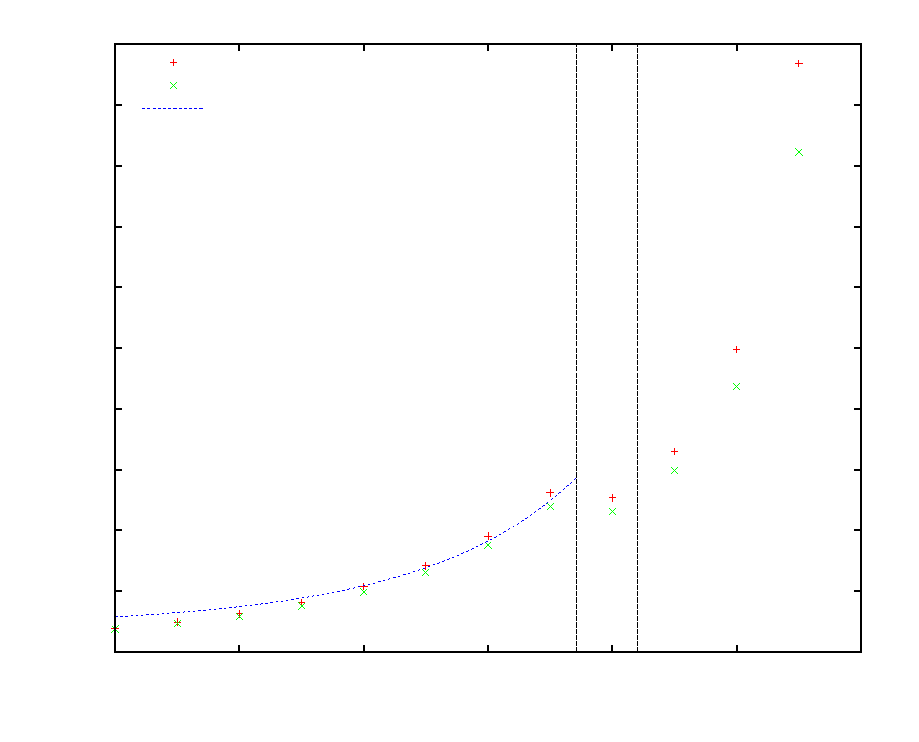
\includegraphics{eos}}%
    \gplfronttext
  \end{picture}%
\endgroup
}
 \caption{Thermische Zustandsgleichung des Systems aus harten Kugeln. Strichlierte vertikale Linien zeigen das 2-Phasengebiet an.}
 \label{fig:zustandsgleichung}
\end{figure} 
Hierbei sei angemerkt, dass Molekulardynamik sowie auch Monte Carlo Simulationen bei sehr geringen Dichten den Phasenraum des Systems nur schlecht abtasten und dass somit die Statistik in diesem Bereich noch fehlerbehaftet sein kann. Bei einer Dichte von $\rho = 1.0 $ gelten die selben Argumente für das 2-Phasengebiet, die schon in Kapitel \ref{sec:paarverteilung} angeführt wurden. 

\subsection{Diffusion}
Des weiteren wurde die Diffusionskonstante $D$ für verschiedene Werte der Dichte $\rho$ berechnet. Sie ergibt sich nach der Green-Kubo-Relation aus dem Integral über die Geschwindigkeits-Autokorrelationsfunktion $C(t)$.
\todo{hier hat neumann nach einem beispiel für geschwindigkeits korrelations funktion o.Ä. gefragt. Genauer Wortlaut der Anmerkung schwer zu entziffern}
\begin{equation}
D = \frac{1}{3}\int_0^{\infty} \langle \vec{v}_i(0)\cdot \vec{v}_i(t)\rangle \text{dt}
\end{equation}
Zum Vergleich wurde die empirische Formel von Speedy \cite{Speedy1987} herangezogen.
\begin{equation}
D = \frac{D_0}{\rho^*}\left(1-\frac{\rho^*}{1.09}\right)\left(1+\rho^{*2}\left(0.4 - 0.83\rho^{*2}\right)\right)
\end{equation}
wobei $\rho^*= \rho \sigma^3$ die reduzierte Dichte ist und $D_0 = \frac{3}{8} \sigma \left(\frac{kT}{\pi m}\right)^{\frac{1}{2}}$. Abbildung \ref{fig:diffusion} zeigt die Diffusionskonstante bei harten Kugeln. Es zeigt sich eine gute Übereinstimmung mit den Ergebnissen von Speedy \cite{Speedy1987}.
\begin{figure}[H]
 \centering
  \resizebox{0.9\textwidth}{!}{% GNUPLOT: LaTeX picture with Postscript
\begingroup
  \makeatletter
  \providecommand\color[2][]{%
    \GenericError{(gnuplot) \space\space\space\@spaces}{%
      Package color not loaded in conjunction with
      terminal option `colourtext'%
    }{See the gnuplot documentation for explanation.%
    }{Either use 'blacktext' in gnuplot or load the package
      color.sty in LaTeX.}%
    \renewcommand\color[2][]{}%
  }%
  \providecommand\includegraphics[2][]{%
    \GenericError{(gnuplot) \space\space\space\@spaces}{%
      Package graphicx or graphics not loaded%
    }{See the gnuplot documentation for explanation.%
    }{The gnuplot epslatex terminal needs graphicx.sty or graphics.sty.}%
    \renewcommand\includegraphics[2][]{}%
  }%
  \providecommand\rotatebox[2]{#2}%
  \@ifundefined{ifGPcolor}{%
    \newif\ifGPcolor
    \GPcolortrue
  }{}%
  \@ifundefined{ifGPblacktext}{%
    \newif\ifGPblacktext
    \GPblacktextfalse
  }{}%
  % define a \g@addto@macro without @ in the name:
  \let\gplgaddtomacro\g@addto@macro
  % define empty templates for all commands taking text:
  \gdef\gplbacktext{}%
  \gdef\gplfronttext{}%
  \makeatother
  \ifGPblacktext
    % no textcolor at all
    \def\colorrgb#1{}%
    \def\colorgray#1{}%
  \else
    % gray or color?
    \ifGPcolor
      \def\colorrgb#1{\color[rgb]{#1}}%
      \def\colorgray#1{\color[gray]{#1}}%
      \expandafter\def\csname LTw\endcsname{\color{white}}%
      \expandafter\def\csname LTb\endcsname{\color{black}}%
      \expandafter\def\csname LTa\endcsname{\color{black}}%
      \expandafter\def\csname LT0\endcsname{\color[rgb]{1,0,0}}%
      \expandafter\def\csname LT1\endcsname{\color[rgb]{0,1,0}}%
      \expandafter\def\csname LT2\endcsname{\color[rgb]{0,0,1}}%
      \expandafter\def\csname LT3\endcsname{\color[rgb]{1,0,1}}%
      \expandafter\def\csname LT4\endcsname{\color[rgb]{0,1,1}}%
      \expandafter\def\csname LT5\endcsname{\color[rgb]{1,1,0}}%
      \expandafter\def\csname LT6\endcsname{\color[rgb]{0,0,0}}%
      \expandafter\def\csname LT7\endcsname{\color[rgb]{1,0.3,0}}%
      \expandafter\def\csname LT8\endcsname{\color[rgb]{0.5,0.5,0.5}}%
    \else
      % gray
      \def\colorrgb#1{\color{black}}%
      \def\colorgray#1{\color[gray]{#1}}%
      \expandafter\def\csname LTw\endcsname{\color{white}}%
      \expandafter\def\csname LTb\endcsname{\color{black}}%
      \expandafter\def\csname LTa\endcsname{\color{black}}%
      \expandafter\def\csname LT0\endcsname{\color{black}}%
      \expandafter\def\csname LT1\endcsname{\color{black}}%
      \expandafter\def\csname LT2\endcsname{\color{black}}%
      \expandafter\def\csname LT3\endcsname{\color{black}}%
      \expandafter\def\csname LT4\endcsname{\color{black}}%
      \expandafter\def\csname LT5\endcsname{\color{black}}%
      \expandafter\def\csname LT6\endcsname{\color{black}}%
      \expandafter\def\csname LT7\endcsname{\color{black}}%
      \expandafter\def\csname LT8\endcsname{\color{black}}%
    \fi
  \fi
  \setlength{\unitlength}{0.0500bp}%
  \begin{picture}(8502.00,6802.00)%
    \gplgaddtomacro\gplbacktext{%
      \csname LTb\endcsname%
      \put(946,704){\makebox(0,0)[r]{\strut{}-0.1}}%
      \put(946,1287){\makebox(0,0)[r]{\strut{} 0}}%
      \put(946,1871){\makebox(0,0)[r]{\strut{} 0.1}}%
      \put(946,2454){\makebox(0,0)[r]{\strut{} 0.2}}%
      \put(946,3037){\makebox(0,0)[r]{\strut{} 0.3}}%
      \put(946,3621){\makebox(0,0)[r]{\strut{} 0.4}}%
      \put(946,4204){\makebox(0,0)[r]{\strut{} 0.5}}%
      \put(946,4787){\makebox(0,0)[r]{\strut{} 0.6}}%
      \put(946,5370){\makebox(0,0)[r]{\strut{} 0.7}}%
      \put(946,5954){\makebox(0,0)[r]{\strut{} 0.8}}%
      \put(946,6537){\makebox(0,0)[r]{\strut{} 0.9}}%
      \put(1078,484){\makebox(0,0){\strut{} 0.2}}%
      \put(2249,484){\makebox(0,0){\strut{} 0.4}}%
      \put(3420,484){\makebox(0,0){\strut{} 0.6}}%
      \put(4592,484){\makebox(0,0){\strut{} 0.8}}%
      \put(5763,484){\makebox(0,0){\strut{} 1}}%
      \put(6934,484){\makebox(0,0){\strut{} 1.2}}%
      \put(8105,484){\makebox(0,0){\strut{} 1.4}}%
      \put(176,3620){\rotatebox{-270}{\makebox(0,0){\strut{}$D$}}}%
      \put(4591,154){\makebox(0,0){\strut{}$\rho $}}%
    }%
    \gplgaddtomacro\gplfronttext{%
      \csname LTb\endcsname%
      \put(7118,6364){\makebox(0,0)[r]{\strut{}Simulation}}%
      \csname LTb\endcsname%
      \put(7118,6144){\makebox(0,0)[r]{\strut{}Theorie}}%
    }%
    \gplbacktext
    \put(0,0){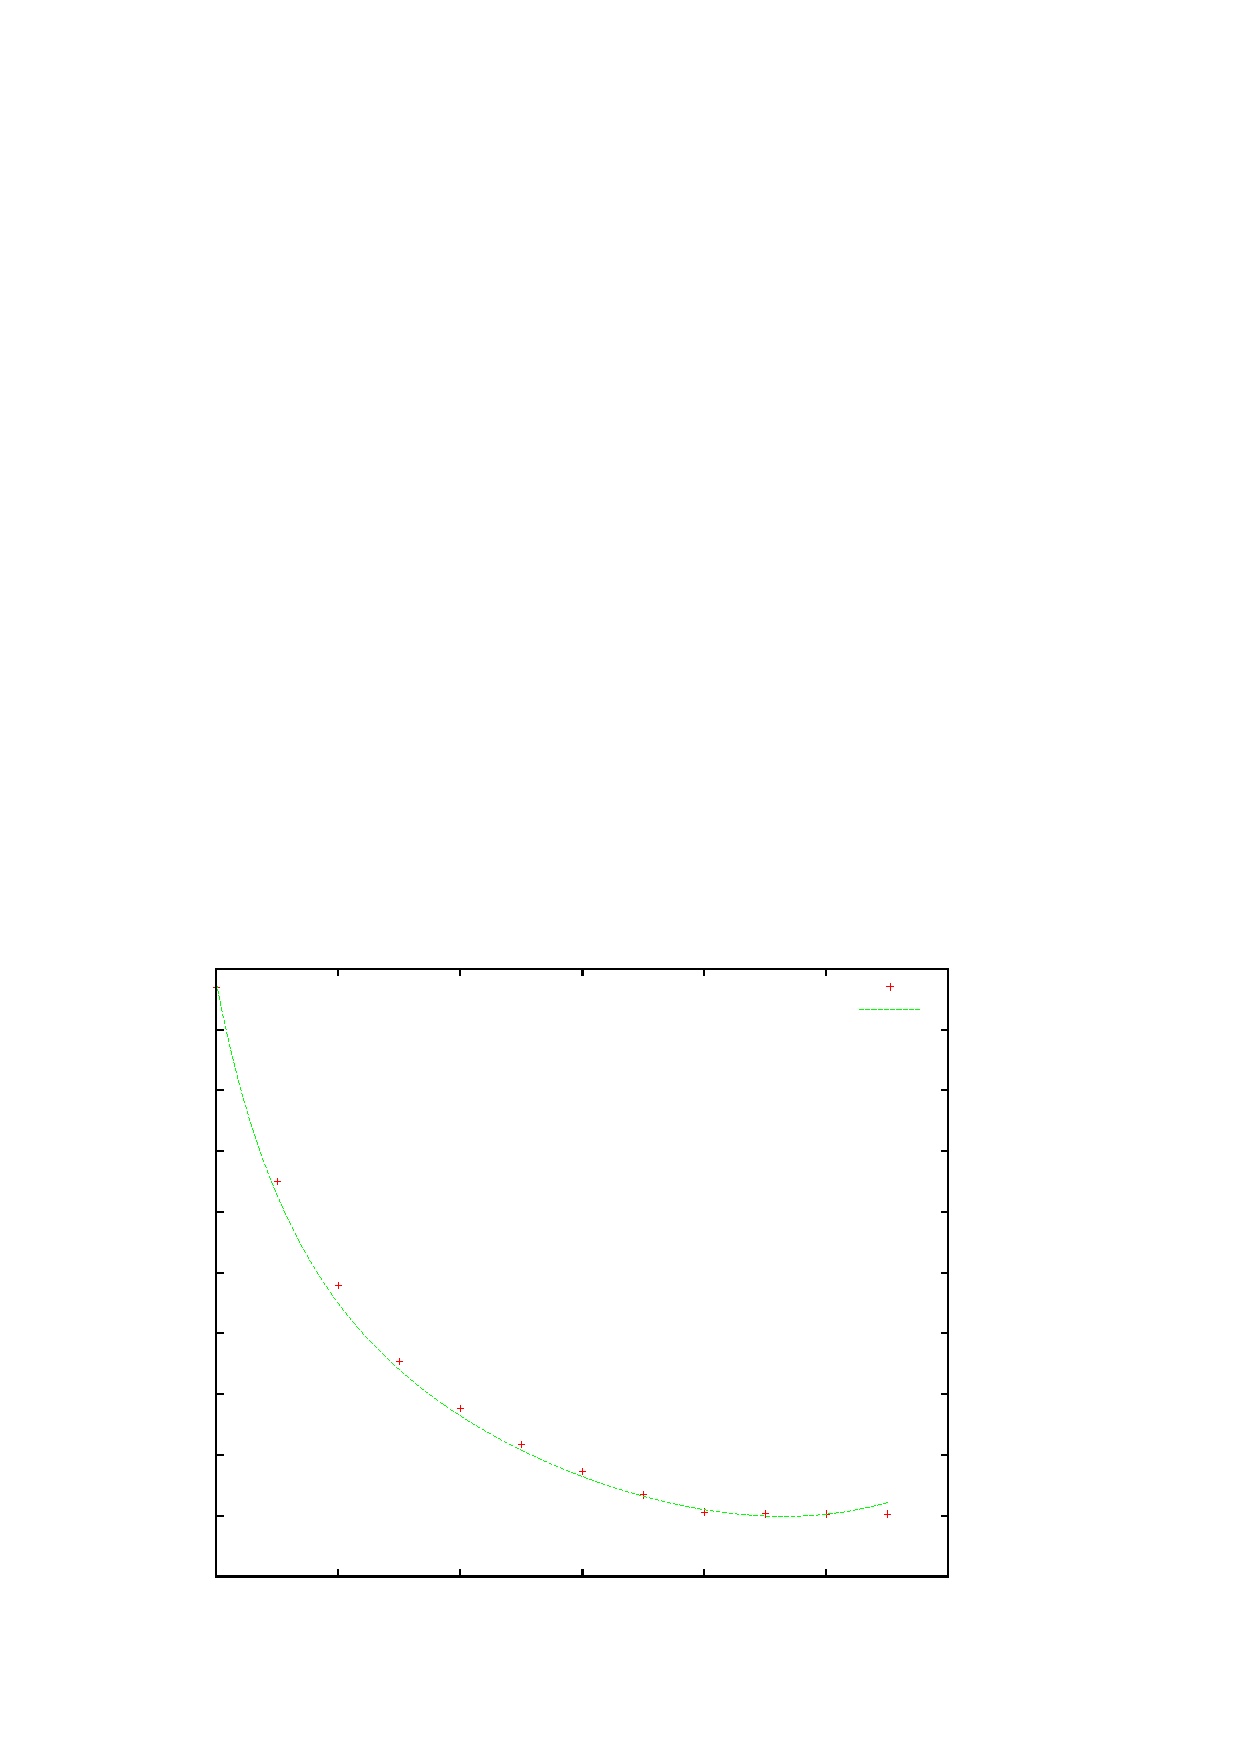
\includegraphics{diffusion}}%
    \gplfronttext
  \end{picture}%
\endgroup
}
 \caption{Diffusionskonstante bei harten Kugeln}
 \label{fig:diffusion}
\end{figure} 
Zur Veranschaulichung zeigen Abbildungen \ref{fig:autocorr-fluid} und \ref{fig:autocorr-solid} nun noch die Geschwindigkeits-Autokorrelationsfunktionen für jeweils eine Dichte der fluiden bzw. festen Phase. Während die Autokorrelationsfunktion in der fluiden Phase exponentiell abfällt, wird sie in der festen Phase negativ bevor sie gegen 0 konvertiert. Das rührt daher, dass die einzelnen Kugeln im Kristall nur um ihre mittlere Position schwingen und nicht durch den Kristall diffundieren. Dies sieht man auch anhand von Abbildung \ref{fig:diffusion} - die Diffusionskonstante fällt im Festkörper auf 0. 

\begin{figure}[H]
 \centering
  \resizebox{0.9\textwidth}{!}{% GNUPLOT: LaTeX picture with Postscript
\begingroup
  \makeatletter
  \providecommand\color[2][]{%
    \GenericError{(gnuplot) \space\space\space\@spaces}{%
      Package color not loaded in conjunction with
      terminal option `colourtext'%
    }{See the gnuplot documentation for explanation.%
    }{Either use 'blacktext' in gnuplot or load the package
      color.sty in LaTeX.}%
    \renewcommand\color[2][]{}%
  }%
  \providecommand\includegraphics[2][]{%
    \GenericError{(gnuplot) \space\space\space\@spaces}{%
      Package graphicx or graphics not loaded%
    }{See the gnuplot documentation for explanation.%
    }{The gnuplot epslatex terminal needs graphicx.sty or graphics.sty.}%
    \renewcommand\includegraphics[2][]{}%
  }%
  \providecommand\rotatebox[2]{#2}%
  \@ifundefined{ifGPcolor}{%
    \newif\ifGPcolor
    \GPcolortrue
  }{}%
  \@ifundefined{ifGPblacktext}{%
    \newif\ifGPblacktext
    \GPblacktextfalse
  }{}%
  % define a \g@addto@macro without @ in the name:
  \let\gplgaddtomacro\g@addto@macro
  % define empty templates for all commands taking text:
  \gdef\gplbacktext{}%
  \gdef\gplfronttext{}%
  \makeatother
  \ifGPblacktext
    % no textcolor at all
    \def\colorrgb#1{}%
    \def\colorgray#1{}%
  \else
    % gray or color?
    \ifGPcolor
      \def\colorrgb#1{\color[rgb]{#1}}%
      \def\colorgray#1{\color[gray]{#1}}%
      \expandafter\def\csname LTw\endcsname{\color{white}}%
      \expandafter\def\csname LTb\endcsname{\color{black}}%
      \expandafter\def\csname LTa\endcsname{\color{black}}%
      \expandafter\def\csname LT0\endcsname{\color[rgb]{1,0,0}}%
      \expandafter\def\csname LT1\endcsname{\color[rgb]{0,1,0}}%
      \expandafter\def\csname LT2\endcsname{\color[rgb]{0,0,1}}%
      \expandafter\def\csname LT3\endcsname{\color[rgb]{1,0,1}}%
      \expandafter\def\csname LT4\endcsname{\color[rgb]{0,1,1}}%
      \expandafter\def\csname LT5\endcsname{\color[rgb]{1,1,0}}%
      \expandafter\def\csname LT6\endcsname{\color[rgb]{0,0,0}}%
      \expandafter\def\csname LT7\endcsname{\color[rgb]{1,0.3,0}}%
      \expandafter\def\csname LT8\endcsname{\color[rgb]{0.5,0.5,0.5}}%
    \else
      % gray
      \def\colorrgb#1{\color{black}}%
      \def\colorgray#1{\color[gray]{#1}}%
      \expandafter\def\csname LTw\endcsname{\color{white}}%
      \expandafter\def\csname LTb\endcsname{\color{black}}%
      \expandafter\def\csname LTa\endcsname{\color{black}}%
      \expandafter\def\csname LT0\endcsname{\color{black}}%
      \expandafter\def\csname LT1\endcsname{\color{black}}%
      \expandafter\def\csname LT2\endcsname{\color{black}}%
      \expandafter\def\csname LT3\endcsname{\color{black}}%
      \expandafter\def\csname LT4\endcsname{\color{black}}%
      \expandafter\def\csname LT5\endcsname{\color{black}}%
      \expandafter\def\csname LT6\endcsname{\color{black}}%
      \expandafter\def\csname LT7\endcsname{\color{black}}%
      \expandafter\def\csname LT8\endcsname{\color{black}}%
    \fi
  \fi
  \setlength{\unitlength}{0.0500bp}%
  \begin{picture}(8502.00,6802.00)%
    \gplgaddtomacro\gplbacktext{%
      \csname LTb\endcsname%
      \put(946,704){\makebox(0,0)[r]{\strut{}-0.5}}%
      \put(946,1537){\makebox(0,0)[r]{\strut{} 0}}%
      \put(946,2371){\makebox(0,0)[r]{\strut{} 0.5}}%
      \put(946,3204){\makebox(0,0)[r]{\strut{} 1}}%
      \put(946,4037){\makebox(0,0)[r]{\strut{} 1.5}}%
      \put(946,4870){\makebox(0,0)[r]{\strut{} 2}}%
      \put(946,5704){\makebox(0,0)[r]{\strut{} 2.5}}%
      \put(946,6537){\makebox(0,0)[r]{\strut{} 3}}%
      \put(1078,484){\makebox(0,0){\strut{} 0}}%
      \put(1956,484){\makebox(0,0){\strut{} 1}}%
      \put(2835,484){\makebox(0,0){\strut{} 2}}%
      \put(3713,484){\makebox(0,0){\strut{} 3}}%
      \put(4592,484){\makebox(0,0){\strut{} 4}}%
      \put(5470,484){\makebox(0,0){\strut{} 5}}%
      \put(6348,484){\makebox(0,0){\strut{} 6}}%
      \put(7227,484){\makebox(0,0){\strut{} 7}}%
      \put(8105,484){\makebox(0,0){\strut{} 8}}%
      \put(176,3620){\rotatebox{-270}{\makebox(0,0){\strut{}$\langle \vec{v}(0) \vec{v}(t)\rangle$}}}%
      \put(4591,154){\makebox(0,0){\strut{}$t $}}%
    }%
    \gplgaddtomacro\gplfronttext{%
      \csname LTb\endcsname%
      \put(7118,6364){\makebox(0,0)[r]{\strut{}$\rho = 0.4$}}%
    }%
    \gplbacktext
    \put(0,0){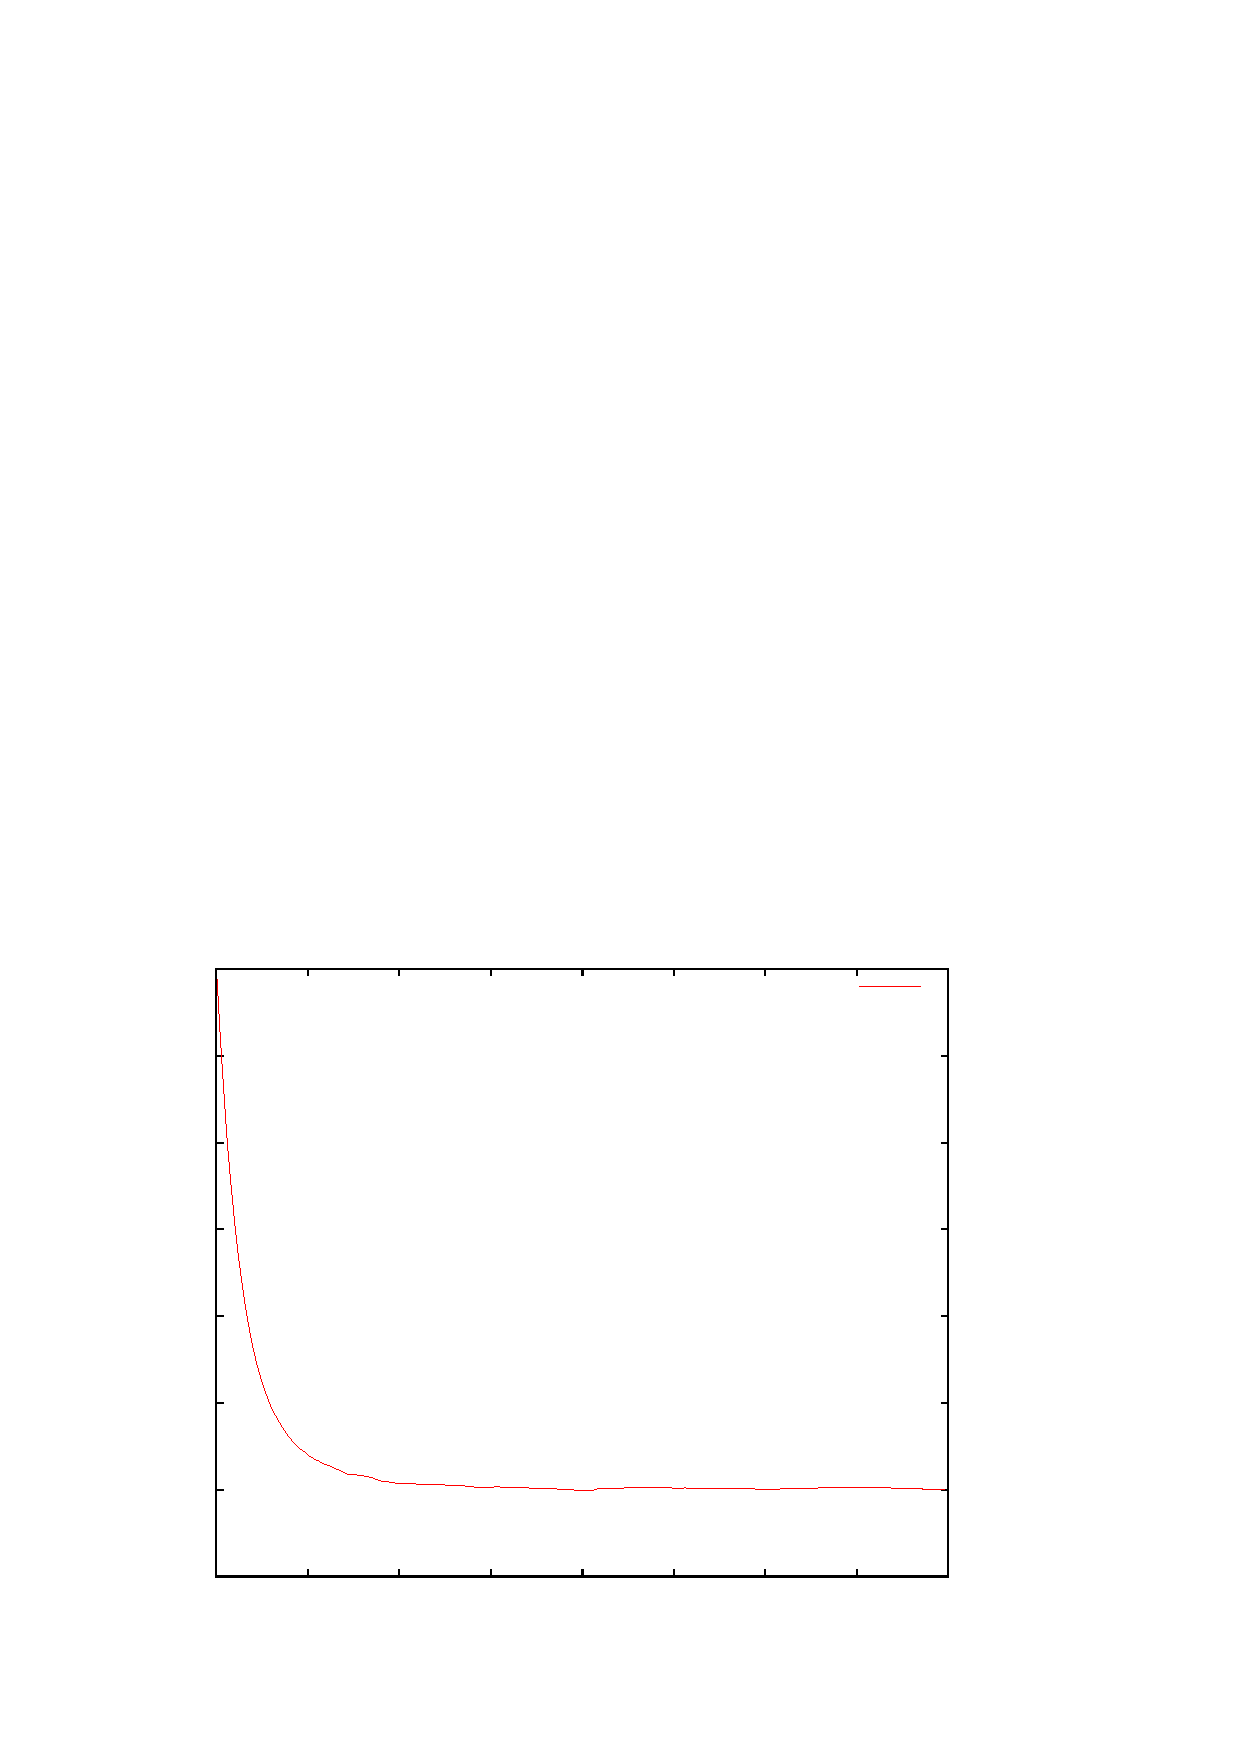
\includegraphics{./autocorrelation-fluid}}%
    \gplfronttext
  \end{picture}%
\endgroup
}
 \caption{Geschwindigkeits-Autokorrelationsfunktion $C(t)$ in der fluiden Phase bei $\rho = 0.4$}
 \label{fig:autocorr-fluid}
\end{figure} 

\begin{figure}[H]
 \centering
  \resizebox{0.9\textwidth}{!}{% GNUPLOT: LaTeX picture with Postscript
\begingroup
  \makeatletter
  \providecommand\color[2][]{%
    \GenericError{(gnuplot) \space\space\space\@spaces}{%
      Package color not loaded in conjunction with
      terminal option `colourtext'%
    }{See the gnuplot documentation for explanation.%
    }{Either use 'blacktext' in gnuplot or load the package
      color.sty in LaTeX.}%
    \renewcommand\color[2][]{}%
  }%
  \providecommand\includegraphics[2][]{%
    \GenericError{(gnuplot) \space\space\space\@spaces}{%
      Package graphicx or graphics not loaded%
    }{See the gnuplot documentation for explanation.%
    }{The gnuplot epslatex terminal needs graphicx.sty or graphics.sty.}%
    \renewcommand\includegraphics[2][]{}%
  }%
  \providecommand\rotatebox[2]{#2}%
  \@ifundefined{ifGPcolor}{%
    \newif\ifGPcolor
    \GPcolortrue
  }{}%
  \@ifundefined{ifGPblacktext}{%
    \newif\ifGPblacktext
    \GPblacktextfalse
  }{}%
  % define a \g@addto@macro without @ in the name:
  \let\gplgaddtomacro\g@addto@macro
  % define empty templates for all commands taking text:
  \gdef\gplbacktext{}%
  \gdef\gplfronttext{}%
  \makeatother
  \ifGPblacktext
    % no textcolor at all
    \def\colorrgb#1{}%
    \def\colorgray#1{}%
  \else
    % gray or color?
    \ifGPcolor
      \def\colorrgb#1{\color[rgb]{#1}}%
      \def\colorgray#1{\color[gray]{#1}}%
      \expandafter\def\csname LTw\endcsname{\color{white}}%
      \expandafter\def\csname LTb\endcsname{\color{black}}%
      \expandafter\def\csname LTa\endcsname{\color{black}}%
      \expandafter\def\csname LT0\endcsname{\color[rgb]{1,0,0}}%
      \expandafter\def\csname LT1\endcsname{\color[rgb]{0,1,0}}%
      \expandafter\def\csname LT2\endcsname{\color[rgb]{0,0,1}}%
      \expandafter\def\csname LT3\endcsname{\color[rgb]{1,0,1}}%
      \expandafter\def\csname LT4\endcsname{\color[rgb]{0,1,1}}%
      \expandafter\def\csname LT5\endcsname{\color[rgb]{1,1,0}}%
      \expandafter\def\csname LT6\endcsname{\color[rgb]{0,0,0}}%
      \expandafter\def\csname LT7\endcsname{\color[rgb]{1,0.3,0}}%
      \expandafter\def\csname LT8\endcsname{\color[rgb]{0.5,0.5,0.5}}%
    \else
      % gray
      \def\colorrgb#1{\color{black}}%
      \def\colorgray#1{\color[gray]{#1}}%
      \expandafter\def\csname LTw\endcsname{\color{white}}%
      \expandafter\def\csname LTb\endcsname{\color{black}}%
      \expandafter\def\csname LTa\endcsname{\color{black}}%
      \expandafter\def\csname LT0\endcsname{\color{black}}%
      \expandafter\def\csname LT1\endcsname{\color{black}}%
      \expandafter\def\csname LT2\endcsname{\color{black}}%
      \expandafter\def\csname LT3\endcsname{\color{black}}%
      \expandafter\def\csname LT4\endcsname{\color{black}}%
      \expandafter\def\csname LT5\endcsname{\color{black}}%
      \expandafter\def\csname LT6\endcsname{\color{black}}%
      \expandafter\def\csname LT7\endcsname{\color{black}}%
      \expandafter\def\csname LT8\endcsname{\color{black}}%
    \fi
  \fi
  \setlength{\unitlength}{0.0500bp}%
  \begin{picture}(8502.00,6802.00)%
    \gplgaddtomacro\gplbacktext{%
      \csname LTb\endcsname%
      \put(946,704){\makebox(0,0)[r]{\strut{}-0.5}}%
      \put(946,1537){\makebox(0,0)[r]{\strut{} 0}}%
      \put(946,2371){\makebox(0,0)[r]{\strut{} 0.5}}%
      \put(946,3204){\makebox(0,0)[r]{\strut{} 1}}%
      \put(946,4037){\makebox(0,0)[r]{\strut{} 1.5}}%
      \put(946,4870){\makebox(0,0)[r]{\strut{} 2}}%
      \put(946,5704){\makebox(0,0)[r]{\strut{} 2.5}}%
      \put(946,6537){\makebox(0,0)[r]{\strut{} 3}}%
      \put(1078,484){\makebox(0,0){\strut{} 0}}%
      \put(2483,484){\makebox(0,0){\strut{} 0.1}}%
      \put(3889,484){\makebox(0,0){\strut{} 0.2}}%
      \put(5294,484){\makebox(0,0){\strut{} 0.3}}%
      \put(6700,484){\makebox(0,0){\strut{} 0.4}}%
      \put(8105,484){\makebox(0,0){\strut{} 0.5}}%
      \put(176,3620){\rotatebox{-270}{\makebox(0,0){\strut{}$ C(t) = \langle \vec{v}(0) \vec{v}(t) \rangle$}}}%
      \put(4591,154){\makebox(0,0){\strut{}$t $}}%
    }%
    \gplgaddtomacro\gplfronttext{%
      \csname LTb\endcsname%
      \put(7118,6364){\makebox(0,0)[r]{\strut{}$\rho = 1.1$}}%
    }%
    \gplbacktext
    \put(0,0){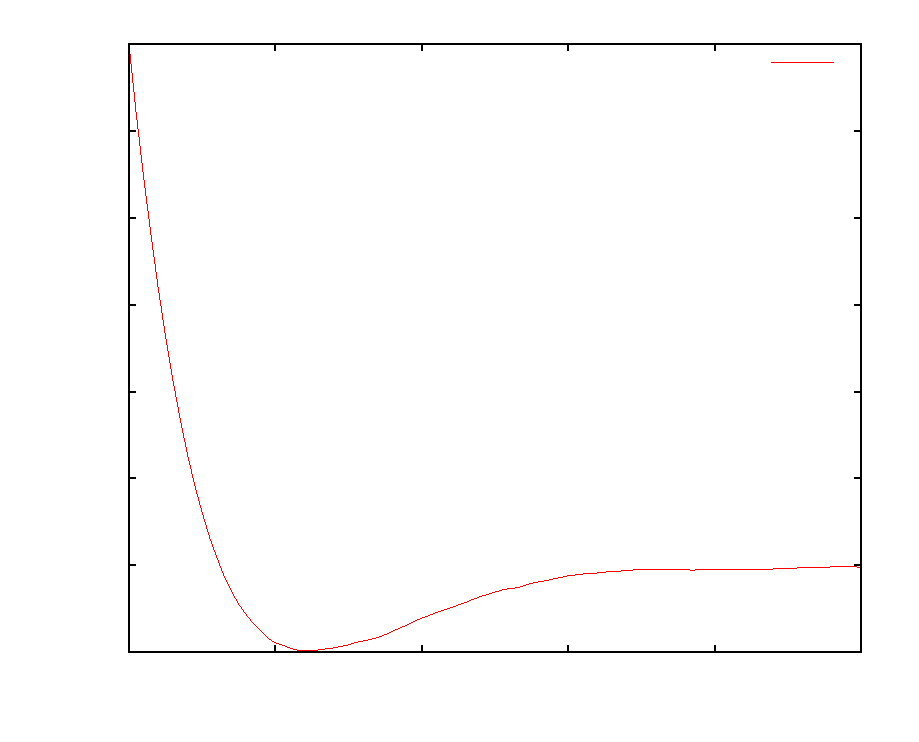
\includegraphics{./autocorrelation-solid}}%
    \gplfronttext
  \end{picture}%
\endgroup
}
 \caption{Geschwindigkeits-Autokorrelationsfunktion $C(t)$ in der festen Phase bei $\rho = 1.1$}
 \label{fig:autocorr-solid}
\end{figure} 
  

\subsection{Freie Bewegungszeiten}
Anschließend wurden noch die freien Bewegungszeiten --- also die Zeiten zwischen zwei Stößen --- untersucht und deren Wahrscheinlichkeitsverteilung analysiert. Bei geringen Dichten kann man molekulares Chaos annehmen und kommt somit zu dem Schluss, dass die Wahrscheinlichkeitsverteilung $p(\tau)$ einem exponentiellen Abfall folgt \cite{Wiegel1976}.

\begin{equation}
p(\tau) = c\cdot e^{-\frac{\tau}{\tau_0}}
\end{equation} 
wobei $c$ nur eine Normierungskonstante ist, sodass $\int_0^{\infty} p(\tau) \text{d}\tau = 1$ -- demnach ist $C = \frac{1}{\tau_0}$. Um dies zu überprüfen und den Parameter $\tau_0$ zu bestimmen, welcher von der Dichte $\rho$ abhängt, wurde der Logarithmus der Wahrscheinlichkeitsverteilung $p(\tau)$ an eine lineare Funktion $f(\tau) = a\cdot \tau + b$ angepasst. Abbildung \ref{fig:collisionfit} zeigt die Wahrscheinlichkeitsverteilung bei einer Dichte von $\rho = 0.6$ und soll zur Veranschaulichung der Durchführung der Bestimmung der Konstante $\tau_0$ dienen. Es sei angemerkt, dass die Werte für $\tau > 0.008$ schon so weit auf 0 herabgefallen sind, dass sie nicht mehr für die statistische Auswertung herangezogen werden konnten. 

\begin{figure}[H]
 \centering
  \resizebox{0.9\textwidth}{!}{% GNUPLOT: LaTeX picture with Postscript
\begingroup
  \makeatletter
  \providecommand\color[2][]{%
    \GenericError{(gnuplot) \space\space\space\@spaces}{%
      Package color not loaded in conjunction with
      terminal option `colourtext'%
    }{See the gnuplot documentation for explanation.%
    }{Either use 'blacktext' in gnuplot or load the package
      color.sty in LaTeX.}%
    \renewcommand\color[2][]{}%
  }%
  \providecommand\includegraphics[2][]{%
    \GenericError{(gnuplot) \space\space\space\@spaces}{%
      Package graphicx or graphics not loaded%
    }{See the gnuplot documentation for explanation.%
    }{The gnuplot epslatex terminal needs graphicx.sty or graphics.sty.}%
    \renewcommand\includegraphics[2][]{}%
  }%
  \providecommand\rotatebox[2]{#2}%
  \@ifundefined{ifGPcolor}{%
    \newif\ifGPcolor
    \GPcolortrue
  }{}%
  \@ifundefined{ifGPblacktext}{%
    \newif\ifGPblacktext
    \GPblacktextfalse
  }{}%
  % define a \g@addto@macro without @ in the name:
  \let\gplgaddtomacro\g@addto@macro
  % define empty templates for all commands taking text:
  \gdef\gplbacktext{}%
  \gdef\gplfronttext{}%
  \makeatother
  \ifGPblacktext
    % no textcolor at all
    \def\colorrgb#1{}%
    \def\colorgray#1{}%
  \else
    % gray or color?
    \ifGPcolor
      \def\colorrgb#1{\color[rgb]{#1}}%
      \def\colorgray#1{\color[gray]{#1}}%
      \expandafter\def\csname LTw\endcsname{\color{white}}%
      \expandafter\def\csname LTb\endcsname{\color{black}}%
      \expandafter\def\csname LTa\endcsname{\color{black}}%
      \expandafter\def\csname LT0\endcsname{\color[rgb]{1,0,0}}%
      \expandafter\def\csname LT1\endcsname{\color[rgb]{0,1,0}}%
      \expandafter\def\csname LT2\endcsname{\color[rgb]{0,0,1}}%
      \expandafter\def\csname LT3\endcsname{\color[rgb]{1,0,1}}%
      \expandafter\def\csname LT4\endcsname{\color[rgb]{0,1,1}}%
      \expandafter\def\csname LT5\endcsname{\color[rgb]{1,1,0}}%
      \expandafter\def\csname LT6\endcsname{\color[rgb]{0,0,0}}%
      \expandafter\def\csname LT7\endcsname{\color[rgb]{1,0.3,0}}%
      \expandafter\def\csname LT8\endcsname{\color[rgb]{0.5,0.5,0.5}}%
    \else
      % gray
      \def\colorrgb#1{\color{black}}%
      \def\colorgray#1{\color[gray]{#1}}%
      \expandafter\def\csname LTw\endcsname{\color{white}}%
      \expandafter\def\csname LTb\endcsname{\color{black}}%
      \expandafter\def\csname LTa\endcsname{\color{black}}%
      \expandafter\def\csname LT0\endcsname{\color{black}}%
      \expandafter\def\csname LT1\endcsname{\color{black}}%
      \expandafter\def\csname LT2\endcsname{\color{black}}%
      \expandafter\def\csname LT3\endcsname{\color{black}}%
      \expandafter\def\csname LT4\endcsname{\color{black}}%
      \expandafter\def\csname LT5\endcsname{\color{black}}%
      \expandafter\def\csname LT6\endcsname{\color{black}}%
      \expandafter\def\csname LT7\endcsname{\color{black}}%
      \expandafter\def\csname LT8\endcsname{\color{black}}%
    \fi
  \fi
  \setlength{\unitlength}{0.0500bp}%
  \begin{picture}(8502.00,6802.00)%
    \gplgaddtomacro\gplbacktext{%
      \csname LTb\endcsname%
      \put(1210,704){\makebox(0,0)[r]{\strut{} 0.001}}%
      \put(1210,1537){\makebox(0,0)[r]{\strut{} 0.01}}%
      \put(1210,2371){\makebox(0,0)[r]{\strut{} 0.1}}%
      \put(1210,3204){\makebox(0,0)[r]{\strut{} 1}}%
      \put(1210,4037){\makebox(0,0)[r]{\strut{} 10}}%
      \put(1210,4870){\makebox(0,0)[r]{\strut{} 100}}%
      \put(1210,5704){\makebox(0,0)[r]{\strut{} 1000}}%
      \put(1210,6537){\makebox(0,0)[r]{\strut{} 10000}}%
      \put(1342,484){\makebox(0,0){\strut{} 0}}%
      \put(2093,484){\makebox(0,0){\strut{} 0.002}}%
      \put(2845,484){\makebox(0,0){\strut{} 0.004}}%
      \put(3596,484){\makebox(0,0){\strut{} 0.006}}%
      \put(4348,484){\makebox(0,0){\strut{} 0.008}}%
      \put(5099,484){\makebox(0,0){\strut{} 0.01}}%
      \put(5851,484){\makebox(0,0){\strut{} 0.012}}%
      \put(6602,484){\makebox(0,0){\strut{} 0.014}}%
      \put(7354,484){\makebox(0,0){\strut{} 0.016}}%
      \put(8105,484){\makebox(0,0){\strut{} 0.018}}%
      \put(176,3620){\rotatebox{-270}{\makebox(0,0){\strut{}$\tau$}}}%
      \put(4723,154){\makebox(0,0){\strut{}$p(\tau)$}}%
    }%
    \gplgaddtomacro\gplfronttext{%
      \csname LTb\endcsname%
      \put(7118,6364){\makebox(0,0)[r]{\strut{}Simulation}}%
      \csname LTb\endcsname%
      \put(7118,6144){\makebox(0,0)[r]{\strut{}Linearer Fit}}%
    }%
    \gplbacktext
    \put(0,0){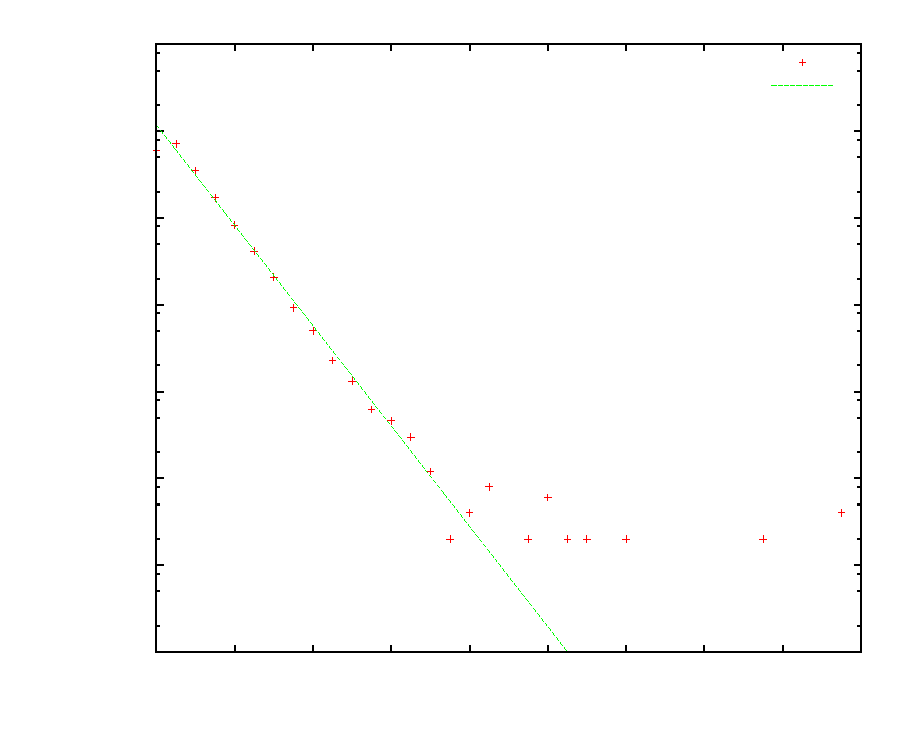
\includegraphics{collisionfitrho06}}%
    \gplfronttext
  \end{picture}%
\endgroup
}
 \caption{Wahrscheinlichkeitsverteilung der freien Bewegungszeiten $p(\tau)$ bei $\rho = 0.6$ in logarithmischer Auftragung und linearer Fit (im Intervall $[0,0.008]$) zur Bestimmung von $\tau_0$}
 \label{fig:collisionfit}
\end{figure} 
Abbildung \ref{fig:flight} zeigt den so berechneten Parameter $\tau_0$ in Abhängigkeit von der Dichte $\rho$. Statt $\tau_0$ wurde allerdings sein Inverses aufgetragen, da sich hier eine annähernd lineare Abhängigkeit von der Dichte im Bereich verdünnter (fluider) Systeme zeigt. Dies ist im Einklang mit den Resultaten von Wiegel und Michels \cite{Wiegel1979}. 

\begin{figure}[H]
 \centering
  \resizebox{0.9\textwidth}{!}{% GNUPLOT: LaTeX picture with Postscript
\begingroup
  \makeatletter
  \providecommand\color[2][]{%
    \GenericError{(gnuplot) \space\space\space\@spaces}{%
      Package color not loaded in conjunction with
      terminal option `colourtext'%
    }{See the gnuplot documentation for explanation.%
    }{Either use 'blacktext' in gnuplot or load the package
      color.sty in LaTeX.}%
    \renewcommand\color[2][]{}%
  }%
  \providecommand\includegraphics[2][]{%
    \GenericError{(gnuplot) \space\space\space\@spaces}{%
      Package graphicx or graphics not loaded%
    }{See the gnuplot documentation for explanation.%
    }{The gnuplot epslatex terminal needs graphicx.sty or graphics.sty.}%
    \renewcommand\includegraphics[2][]{}%
  }%
  \providecommand\rotatebox[2]{#2}%
  \@ifundefined{ifGPcolor}{%
    \newif\ifGPcolor
    \GPcolortrue
  }{}%
  \@ifundefined{ifGPblacktext}{%
    \newif\ifGPblacktext
    \GPblacktextfalse
  }{}%
  % define a \g@addto@macro without @ in the name:
  \let\gplgaddtomacro\g@addto@macro
  % define empty templates for all commands taking text:
  \gdef\gplbacktext{}%
  \gdef\gplfronttext{}%
  \makeatother
  \ifGPblacktext
    % no textcolor at all
    \def\colorrgb#1{}%
    \def\colorgray#1{}%
  \else
    % gray or color?
    \ifGPcolor
      \def\colorrgb#1{\color[rgb]{#1}}%
      \def\colorgray#1{\color[gray]{#1}}%
      \expandafter\def\csname LTw\endcsname{\color{white}}%
      \expandafter\def\csname LTb\endcsname{\color{black}}%
      \expandafter\def\csname LTa\endcsname{\color{black}}%
      \expandafter\def\csname LT0\endcsname{\color[rgb]{1,0,0}}%
      \expandafter\def\csname LT1\endcsname{\color[rgb]{0,1,0}}%
      \expandafter\def\csname LT2\endcsname{\color[rgb]{0,0,1}}%
      \expandafter\def\csname LT3\endcsname{\color[rgb]{1,0,1}}%
      \expandafter\def\csname LT4\endcsname{\color[rgb]{0,1,1}}%
      \expandafter\def\csname LT5\endcsname{\color[rgb]{1,1,0}}%
      \expandafter\def\csname LT6\endcsname{\color[rgb]{0,0,0}}%
      \expandafter\def\csname LT7\endcsname{\color[rgb]{1,0.3,0}}%
      \expandafter\def\csname LT8\endcsname{\color[rgb]{0.5,0.5,0.5}}%
    \else
      % gray
      \def\colorrgb#1{\color{black}}%
      \def\colorgray#1{\color[gray]{#1}}%
      \expandafter\def\csname LTw\endcsname{\color{white}}%
      \expandafter\def\csname LTb\endcsname{\color{black}}%
      \expandafter\def\csname LTa\endcsname{\color{black}}%
      \expandafter\def\csname LT0\endcsname{\color{black}}%
      \expandafter\def\csname LT1\endcsname{\color{black}}%
      \expandafter\def\csname LT2\endcsname{\color{black}}%
      \expandafter\def\csname LT3\endcsname{\color{black}}%
      \expandafter\def\csname LT4\endcsname{\color{black}}%
      \expandafter\def\csname LT5\endcsname{\color{black}}%
      \expandafter\def\csname LT6\endcsname{\color{black}}%
      \expandafter\def\csname LT7\endcsname{\color{black}}%
      \expandafter\def\csname LT8\endcsname{\color{black}}%
    \fi
  \fi
  \setlength{\unitlength}{0.0500bp}%
  \begin{picture}(8502.00,6802.00)%
    \gplgaddtomacro\gplbacktext{%
      \csname LTb\endcsname%
      \put(1078,704){\makebox(0,0)[r]{\strut{} 0}}%
      \put(1078,1287){\makebox(0,0)[r]{\strut{} 500}}%
      \put(1078,1871){\makebox(0,0)[r]{\strut{} 1000}}%
      \put(1078,2454){\makebox(0,0)[r]{\strut{} 1500}}%
      \put(1078,3037){\makebox(0,0)[r]{\strut{} 2000}}%
      \put(1078,3621){\makebox(0,0)[r]{\strut{} 2500}}%
      \put(1078,4204){\makebox(0,0)[r]{\strut{} 3000}}%
      \put(1078,4787){\makebox(0,0)[r]{\strut{} 3500}}%
      \put(1078,5370){\makebox(0,0)[r]{\strut{} 4000}}%
      \put(1078,5954){\makebox(0,0)[r]{\strut{} 4500}}%
      \put(1078,6537){\makebox(0,0)[r]{\strut{} 5000}}%
      \put(1210,484){\makebox(0,0){\strut{} 0}}%
      \put(2271,484){\makebox(0,0){\strut{} 0.2}}%
      \put(3332,484){\makebox(0,0){\strut{} 0.4}}%
      \put(4392,484){\makebox(0,0){\strut{} 0.6}}%
      \put(5453,484){\makebox(0,0){\strut{} 0.8}}%
      \put(6514,484){\makebox(0,0){\strut{} 1}}%
      \put(7575,484){\makebox(0,0){\strut{} 1.2}}%
      \put(176,3620){\rotatebox{-270}{\makebox(0,0){\strut{}$1/\tau_0$}}}%
      \put(4657,154){\makebox(0,0){\strut{}$\rho$}}%
    }%
    \gplgaddtomacro\gplfronttext{%
    }%
    \gplbacktext
    \put(0,0){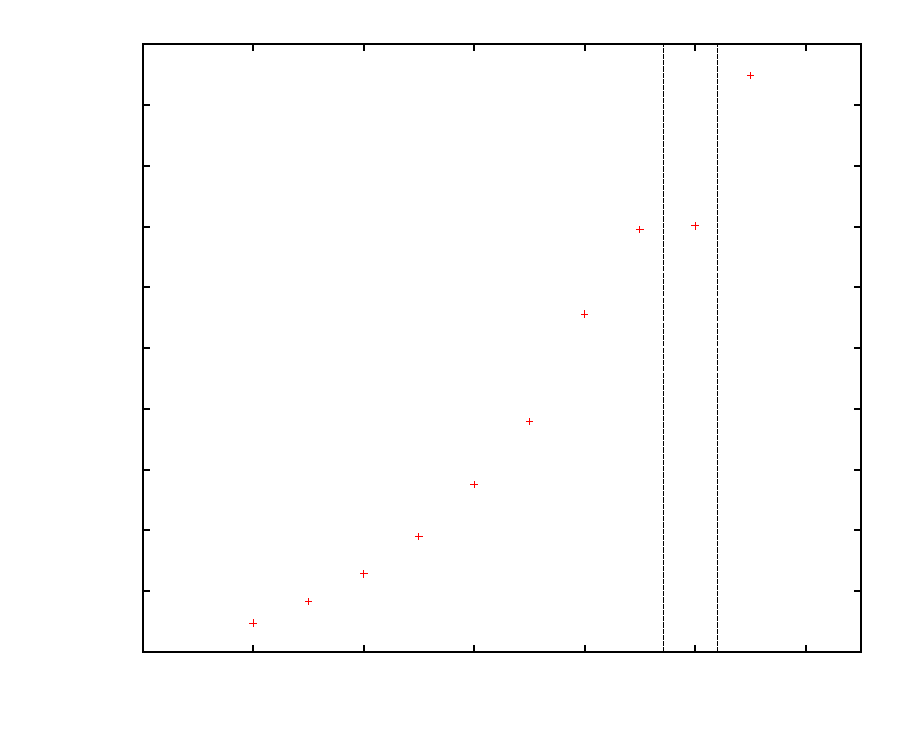
\includegraphics{flighttimes}}%
    \gplfronttext
  \end{picture}%
\endgroup
}
 \caption{Durch linearen Fit bestimmte Konstante $\tau_0$ in Abhängigkeit von $\rho$}
 \label{fig:flight}
\end{figure} 